\clearpage
\newpage
\noindent\\
\thispagestyle{empty}
\begin{center}
\Large
\begin{flushright}
\vspace{17cm} {\Huge \em{ \textbf{\textcolor{ultramarine}{CONFERENCIAS}}}} \\ [0.5cm]
\addcontentsline{toc}{section}{Conferencias}
\end{flushright}
\normalsize
\end{center}

\small
\clearpage
\pagestyle{fancy}
\SetHeader{Conferencias}{\textit{Congreso Interamericano de Estadística}}

\newcommand{\titulo}{algo}
\newcommand{\presentador}{algo}
\newcommand{\lugar}{algo}

%--------------------------------------------------------------------------
\renewcommand{\titulo}{EL CENSO, ELEMENTO FUNDAMENTAL DE UN SISTEMA MODERNO DE ESTADÍSTICAS NACIONALES}
\renewcommand{\presentador}{DR. ALPHONSE L. MACDONALD}
\renewcommand{\lugar}{OFICINA GENERAL DE ESTADÍSTICA (ABS), SURINAME}
\addcontentsline{toc}{subsubsection}{\textbf{CONFERENCIA INAUGURAL:} \titulo. \\\presentador}
\vspace*{1cm}

\begin{center}
\textit{Conferencia inaugural\\}
\bigskip
\textbf{\textcolor{ultramarine}{\titulo \\}}
\bigskip
\textit{\presentador \\}
\bigskip
\scriptsize{\lugar}
\bigskip
\end{center}

\noindent Cada sociedad moderna requiere información estadística, no solo el gobierno para desarrollar sus políticas y programas, sino también la ciudadanía para evaluar el cumplimiento de los programas nacionales, el sector comercial e industrial para desarrollar y evaluar sus inversiones y el sector privado para planificar y establecer el éxito de sus acciones. Esta información se obtiene a través de un sistema de estadísticas nacionales que proviene de diferentes fuentes de información, primordialmente datos administrativos y censos hasta la Segunda Guerra Mundial, y después también las encuestas. En la región latinoamericana se establecieron sistemas estadísticos nacionales gracias a las iniciativas y el apoyo de las organizaciones internacionales, incluso el Instituto Interamericano de Estadística (IASI). En el sistema de estadísticas nacionales el censo tiene una importancia crucial ya que cuenta con una metodología bien establecida, con criterios determinados para medir la validez y confiabilidad de los resultados, así como la cobertura de la población meta. Desde hace unos 40 años se presentaron alternativas al censo. En esta conferencia se revisarán las razones por las cuales surgían las alternativas, sus características y si éstas pueden reemplazar al censo como elemento clave de un sistema de estadísticas nacionales.

\begin{table}[H]
\centering
\begin{tabular}{m{0.25\textwidth}  m{0.7\textwidth}}
\begin{center} 
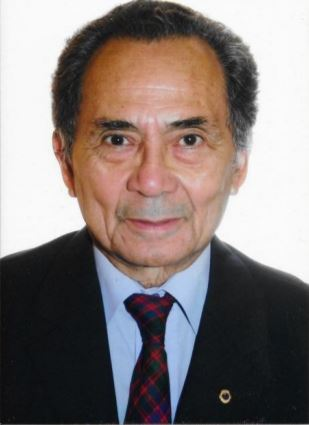
\includegraphics[width=0.2\textwidth]{./fotos/alphonse} \end{center} & 
\noindent \small{Alphonse L. MacDonald, ciudadano de Suriname, Doctor de la Universidad Radboud, Nimega, Países bajos. Especialista en metodología de la investigación, censos, encuestas de hogares y en la planificación económica. Participó en dos proyectos de estadísticas internacionalesinventores: la Encuesta Mundial de Fecundidad (WFS) y el Programa para Desarrollar la Capacidad Nacional de Efectuar Encuestas por Hogares (NHSCP). Ocupó altos cargos técnicos y de representación en las Naciones Unidas en África, América y Europa. Se retiró de la ONU en 2004, pero sigue activo como consultor independiente. Además sigue siendo Consejero Principal (metodología) de la Oficina General de Estadística (ABS) de Suriname.} \\
\end{tabular}
\end{table}

 %--------------------------------------------------------------------------

\newpage
\clearpage
\renewcommand{\titulo}{PENSAMIENTO ESTADÍSTICO: ¿EJE GUÍA EN LOS CURSOS FORMALES DE ESTADÍSTICA? }
\renewcommand{\presentador}{DR. ROBERTO BEHAR GUTIERREZ}
\renewcommand{\lugar}{UNIVERSIDAD DEL VALLE, CALI, COLOMBIA}
\addcontentsline{toc}{subsubsection}{\titulo. \presentador}
\vspace*{1cm}

\begin{center}
\textbf{\textcolor{ultramarine}{\titulo \\}}
\bigskip
\textit{\presentador \\}
\bigskip
\scriptsize{\lugar}
\bigskip
\end{center}

\noindent En su conferencia, el profesor Behar Gutiérrez desarrolla las ideas básicas del llamado “Pensamiento Estadístico” principalmente con el enfoque definido por Wild y Pfannkuch (1999) y lo contrasta con lo que considera la moda del desarrollo de cursos típicos introductorios de Estadística a nivel superior; no obstante que los planteamientos son válidos para la formación en el nivel medio de educación. Plantea como un riesgo el alejarse de la formación holística y sistémica del Pensamiento Estadístico y poner como centro la matemática de la estadística, en lugar del aprendizaje sobre un fenómeno en ambiente de variabilidad e incertidumbre, que es el entorno en el cual surge la naturaleza del razonamiento inductivo de la Estadística. Hace énfasis en la necesidad de dar un giro, del enfoque orientado hacia las herramientas o instrumentos estadísticos, hacia la resolución de verdaderos problemas y advierte que seguir el orden de los temas establecido en el libro de texto, no va en la dirección correcta, pues descontextualiza y fracciona el conocimiento; plantea en su lugar, un enfoque en espiral, en el cual se aborda siempre un problema completo, para el cual la complejidad de su solución va aumentando con cada vuelta de la espiral. Propone ejemplos de cómo se puede materializar este enfoque y recomienda algunas actividades y referencias bibliográficas que ayudan a lograr este propósito. 

\begin{table}[H]
\centering
\begin{tabular}{m{0.25\textwidth}  m{0.7\textwidth}}
\begin{center} 
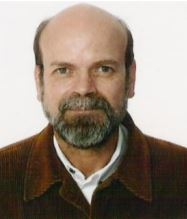
\includegraphics[width=0.2\textwidth]{./fotos/gutierrez} \end{center} & 
\noindent \small{Roberto Behar Gutierrez es profesor titular de la Escuela de Estadística de la Universidad del Valle, Cali, Colombia. Es Licenciado en Educación, con especialidad en Matemáticas, además tiene títulos profesionales en Ingeniería y en Estadística. Es Maestro en Ciencias en Estadística por el Colegio de Posgraduados de Chapingo, México y Doctor en Ciencias Matemáticas por la Universidad Politécnica de Cataluña, Barcelona. Sus actividades de formación en Estadística, han estado centradas especialmente en las carreras pregrado y posgrado de Estadistica, Ingeniería y en la Licenciatura en Educación Matemática. Desde 1979, ha contribuido a la formación de varias generaciones de estadísticos profesionales y a la difusión de la estadística y el pensamiento estadístico en el mundo de habla hispana. El libro “55 Respuestas a dudas típicas en estadística” en coautoría con Pere Grima, de la UPC, Barcelona, publicado por la editorial española Díaz de Santos, ha tenido gran aceptación en todos los países de habla hispana y se espera que muy pronto, esté disponible para el mundo angloparlante. Recientemente escribió en coautoría con Pere Grima y Lluis Marco, el artículo “Twenty-Five Analogies for Explaining Statistical Concepts” publicado por The American Statistician. Este mismo trabajo fue seleccionado y publicado en el libro The Best Writing on Mathematics 2014, por la Princeton Town University Press. Ha sido consultor estadístico en la industria y en el sector público y ha sido miembro del equipo de la Escuela de Ingenieros Industriales de la UPC, con el
cual ha realizado capacitación estadística a ingenieros y profesionales del sector público y privado en Iberoamérica, principalmente a través del enfoque conocido como “Seis Sigma”.} \\
\end{tabular}
\end{table}



 %--------------------------------------------------------------------------

\newpage
\clearpage
\renewcommand{\titulo}{PRINCIPALES DESAFÍOS EN LA RECONSTRUCCIÓN Y AMPLIACIÓN DEL IPC AL ÁMBITO NACIONAL}
\renewcommand{\presentador}{MG. ALEJANDRA CLEMENTE}
\renewcommand{\lugar}{INSTITUTO NACIONAL DE ESTADÍSTICAS Y CENSOS (INDEC), ARGENTINA}
\addcontentsline{toc}{subsubsection}{\titulo. \presentador}
\vspace*{1cm}

\begin{center}
\textbf{\textcolor{ultramarine}{\titulo \\}}
\bigskip
\textit{\presentador \\}
\bigskip
\scriptsize{\lugar}
\bigskip
\end{center}

\noindent El Índice de Precios al Consumidor (IPC) mide la evolución de los precios de una canasta de bienes y servicios representativos del gasto en consumo de los hogares. Junto con otros indicadores de precios constituye un indicador clave para el monitoreo de la economía y como instrumento para la evaluación de la política monetaria. En el año 2013 las estadísticas argentinas recibieron una declaración de censura por parte del Fondo Monetario Internacional a raíz de las inconsistencias detectadas en las mediciones del Índice de Precios al Consumidor (IPC) y el Producto Bruto Interno (PIB). En diciembre de 2015 se suspendió la difusión del calendario del difusión del INDEC hasta tanto se realice una revisión técnica de los distintos operativos estadísticos en el marco de la emergencia estadística establecida a través del Decreto N° 55/2016. En el mes de junio de 2016 se reanudó la publicación del Índice de Precios de Consumo (IPC-GBA). Su publicación requirió una profunda revisión de todos los aspectos involucrados en la construcción del índice desde la revisión de la canasta de bienes y servicios, la estructura de ponderaciones para los distintos ítems que la componen, la muestra de informantes y los procedimientos de cálculo, entre otros. Como resultado de este proceso y luego de distintas visitas técnicas se levantó la declaración de censura a las estadísticas públicas argentinas y fue posible la ampliación de la cobertura del IPC al ámbito nacional, con resultados representativos de todas las regiones del país. \\ \\

\noindent \small{Alejandra Clemente es Licenciada en Estadística de la Universidad Nacional de Rosario y Magíster en Economía de la Universidad Torcuato Di Tella (UTDT). Cuenta con amplia experiencia docente en temas vinculados a probabilidades, estadística y econometría. Especialista en análisis y metodología de índices de precios y core inflation, en diseño y análisis de encuestas, desestacionalización de indicadores económicos, entre otros. Desde 1999 hasta 2007 se desempeñó en las áreas de Índices de Precios de Consumo y Metodología Estadística de INDEC. En el ámbito privado ha trabajado como experta estadística en diversos estudios vinculados al sector energético, agua potable, tabaquismo, sector agroalimentario, entre otros. A partir de diciembre de 2015 se reincorporó al INDEC como Directora de Índices de Precios de Consumo. Tuvo a su cargo la revisión del IPC GBA cuya difusión se reanudó a partir del mes de mayo de 2016 como así también de la ampliación del actual IPC al ámbito nacional cuyos resultados comenzaron a difundirse a partir del mes de junio de 2017. Actualmente se encuentra a cargo de la Dirección Nacional de Estadísticas de Condiciones de Vida.} \\



 %--------------------------------------------------------------------------
\newpage
\clearpage
\renewcommand{\titulo}{IMPACTO DE LOS ERRORES DE MEDICIÓN EN LA EVALUACIÓN DE LA CAPACIDAD DE PROCESOS MULTIVARIADOS}
\renewcommand{\presentador}{DRA. DANIELA DIANDA}
\renewcommand{\lugar}{UNIVERSIDAD NACIONAL DE ROSARIO, ARGENTINA}
\addcontentsline{toc}{subsubsection}{\titulo. \presentador}
\vspace*{1cm}

\begin{center}
\textbf{\textcolor{ultramarine}{\titulo \\}}
\bigskip
\textit{\presentador \\}
\bigskip
\scriptsize{\lugar}
\bigskip
\end{center}

\noindent El crecimiento de los avances tecnológicos ocurridos en las últimas décadas y la sofisticación de los procesos traen como consecuencia la necesidad de evaluar la calidad de productos y servicios con un enfoque multidimensional integrador, que considere el comportamiento de cada una de las variables que la definen, sin ignorar la estructura de correlación entre ellas. El análisis multivariado de capacidad de procesos ha recibido considerable atención en los últimos años, proponiéndose distintas alternativas de índices, de los cuales se desconocen en muchos casos sus propiedades teóricas y/o la validez de su aplicación en contextos prácticos particulares. En esta conferencia se presentan los principales resultados del estudio de algunos de los índices de capacidad de procesos multivariados más divulgados, incluyendo la evaluación del impacto que los errores de medición pueden tener sobre los mismos. La importancia de las conclusiones obtenidas deriva de la alta frecuencia con la que pueden aparecer estos errores en el contexto de la automatización de los procesos y del registro de las mediciones cuantitativas, debiéndose poner el énfasis en la calibración de los sistemas de medición antes de cualquier evaluación de capacidad. El crecimiento de los avances tecnológicos ocurridos en las últimas décadas y la sofisticación de los procesos traen como consecuencia la necesidad de evaluar la calidad de productos y servicios con un enfoque multidimensional integrador, que considere el comportamiento de cada una de las variables que la definen, sin ignorar la estructura de correlación entre ellas. El análisis multivariado de capacidad de procesos ha recibido considerable atención en los últimos años, proponiéndose distintas alternativas de índices, de los cuales se desconocen en muchos casos sus propiedades teóricas y/o la validez de su aplicación en contextos prácticos particulares. En esta conferencia se presentan los principales resultados del estudio de algunos de los índices de capacidad de procesos multivariados más divulgados, incluyendo la evaluación del impacto que los errores de medición pueden tener sobre los mismos. La importancia de las conclusiones obtenidas deriva de la alta frecuencia con la que pueden aparecer estos errores en el contexto de la automatización de los procesos y del registro de las mediciones cuantitativas, debiéndose poner el énfasis en la calibración de los sistemas de medición antes de cualquier evaluación de capacidad.

\begin{table}[H]
\centering
\begin{tabular}{m{0.25\textwidth}  m{0.7\textwidth}}
\begin{center} 
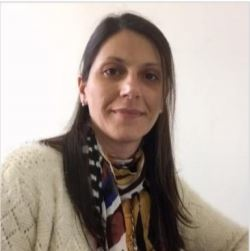
\includegraphics[width=0.2\textwidth]{./fotos/dani} \end{center} & 
\noindent \small{Dra. Daniela Dianda. Licenciada en Estadística y Doctora en Estadística (UNR). Actualmente es profesora en la Licenciatura en Estadística (Facultad de Ciencias Económicas y Estadística, UNR) y becaria posdoctoral de CONICET. Su principal área de interés en investigación son los métodos
estadísticos aplicados a la mejora de la calidad y la productividad. Participa desde el año 2007 en equipos de investigación dedicados a
esta temática, tanto en el marco del programa de incentivos, como en proyectos de vinculación tecnológica.} \\
\end{tabular}
\end{table}

 %--------------------------------------------------------------------------
\newpage
\clearpage
\renewcommand{\titulo}{EL IASI: ORIGEN, OBJETIVOS Y ACTIVIDADES RELEVANTES}
\renewcommand{\presentador}{DR. EVELIO O. FABBRONI}
\renewcommand{\lugar}{INSTITUTO INTERAMERICANO DE ESTADISTICA (IASI)}
\addcontentsline{toc}{subsubsection}{\titulo. \presentador}
\vspace*{1cm}

\begin{center}
\textbf{\textcolor{ultramarine}{\titulo \\}}
\bigskip
\textit{\presentador \\}
\bigskip
\scriptsize{\lugar}
\bigskip
\end{center}

\noindent El Instituto Interamericano de Estadística (IASI), fundado en 1940 con el propósito de promover el desarrollo de la estadística en la región americana, ha generado y ejecutado a través de los años una serie de programas que han contribuido significativamente al cumplimiento de sus objetivos. Se hará una reseña de las actividades más relevantes del Instituto, destinadas a distintos sectores de la comunidad estadística, destacándose su cooperación con instituciones nacionales y organizaciones internacionales.

\begin{table}[H]
\centering
\begin{tabular}{m{0.25\textwidth}  m{0.7\textwidth}}
\begin{center} 
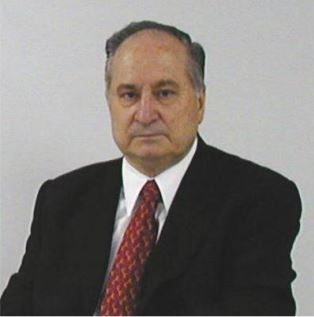
\includegraphics[width=0.2\textwidth]{./fotos/fabbroni} \end{center} & 
\noindent \small{Evelio O. Fabbroni. Estadístico Matemático (Universidad Nacional del Litoral, Rosario, Argentina, 1951). Master of Philosophpy-Ph.D. Candidate (The George Washington University, Washington, DC, USA, 1971). Profesor en universidades de varios países de la región y en el Centro Interamericano de Enseñanza de Estadística (CIENES). Dirige la Oficina Permanente del IASI desde 1981, actualmente como Director Ejecutivo.} \\
\end{tabular}
\end{table}



 %--------------------------------------------------------------------------

\newpage
\clearpage
\renewcommand{\titulo}{MODELANDO NOTICIAS COMPLEJAS Y SOSPECHOSAS: UN ENFOQUE MULTI-TÉCNICA Y MULTIVARIADO}
\renewcommand{\presentador}{DR. JOSÉ LUIS GUERRERO-CUSUMANO}
\renewcommand{\lugar}{GEORGETOWN UNIVERSITY, USA}
\addcontentsline{toc}{subsubsection}{\titulo. \presentador}
\vspace*{1cm}

\begin{center}
\textbf{\textcolor{ultramarine}{\titulo \\}}
\bigskip
\textit{\presentador \\}
\bigskip
\scriptsize{\lugar}
\bigskip
\end{center}

\noindent La veracidad se refiere a la integridad y exactitud de los datos, incluyendo la incertidumbre de los mismos. La veracidad de los datos a menudo se pasa por alto en la minería de textos. El descubrimiento de la verdad es inferir simultáneamente sobre "la verdad y la confiabilidad de la fuente" de los datos. Una fuente es confiable si proporciona muchas piezas de información verdadera, por lo tanto, una información es probable que sea verdadera si es proporcionada por muchas fuentes confiables. La intención de la conferencia es proporcionar un marco multivariado a los investigadores y profesionales para analizar las noticias sospechosas o complejas a través de distintos enfoques avanzados: distribuciones de probabilidad (Generalized Gamma Poisson model), el modelado predictivo (Multiple Negative Binomial Regression), análisis de series temporales (enfoque de correlación cruzada) y gráficos multivariados de control, técnicas multivariantes (Análisis Conjunto de Correlaciones, Análisis de Correspondencia), etc. Este enfoque sistemático pretende ayudar a los investigadores y profesionales para arrojar alguna luz sobre el complejo ámbito de la veracidad. 

\begin{table}[H]
\centering
\begin{tabular}{m{0.25\textwidth}  m{0.7\textwidth}}
\begin{center} 
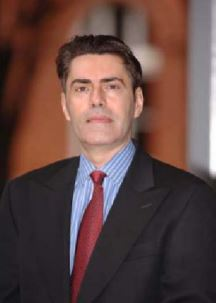
\includegraphics[width=0.2\textwidth]{./fotos/cusumano} \end{center} & 
\noindent \small{El Dr. Guerrero-Cusumano es Profesor Titular de la Escuela de Negocios de la Universidad de Georgetown. Tiene un doctorado en Ingeniería Industrial de la Universidad de Illinois y una Maestría en Ciencias de Estadísticas del Departamento de la Universidad de Illinois Matemáticas. Es también
Estadístico de la Facultad de Ciencias Económicas, Universidad de Rosario, Argentina. Prof. Guerrero-Cusumano ha sido miembro de la facultad en Georgetown
desde 1989 en la Escuela de Negocios. Es el director académico de la International Corporate Maestría en la Escuela de Negocios de la Universidad de Georgetown (2012-2017) y fue director del Instituto Internacional de Gobierno, administración y Política de Georgetown University. En 2008, el profesor Guerrero Cusumano fue galardonado con un Doctorado Honorario en Administración por la Universidad Ovidius (Rumanía) y elegido miembro de la Judge Business School de la Universidad de Cambridge, Gran Bretaña. En 2017, fue reconocido por el Instituto Internacional para la Gestión del Conocimiento Aplicado, con el Premio Académico para un Investigador Distinguido. Entre sus áreas de investigación están el análisis de grandes y pequeños de datos, minería de datos, minería de textos, Negocios Internacionales, Responsabilidad Social, Previsión de negocios, Six Sigma y Mejora de la Calidad. En 2017, fue el co-presidente de la Conferencia Internacional sobre la Organización Responsable en el Contexto Global. Ha publicado más de cincuenta artículos en revistas importantes.} \\
\end{tabular}
\end{table}



 %--------------------------------------------------------------------------

\newpage
\clearpage
\renewcommand{\titulo}{ENSEÑANZA DE LA ESTADÍSTICA: LA FORMACIÓN DEL PROFESORADO ANTE EL RETO DE LA EDUCACIÓN CRÍTICA}
\renewcommand{\presentador}{PROF. MARÍA INÉS HERRERA}
\renewcommand{\lugar}{UNIVERSIDAD NACIONAL DEL LITORAL, ARGENTINA}
\addcontentsline{toc}{subsubsection}{\titulo. \presentador}
\vspace*{1cm}

\begin{center}
\textbf{\textcolor{ultramarine}{\titulo \\}}
\bigskip
\textit{\presentador \\}
\bigskip
\scriptsize{\lugar}
\bigskip
\end{center}

\noindent En esta conferencia, la profesora Herrera reflexiona sobre distintas iniciativas dirigidas a la formación de los profesores para promover y fortalecer la enseñanza de la Estadística, en las que ha participado. Asume que existen dificultades para desarrollar la alfabetización, el razonamiento y el pensamiento estadístico, competencias en que se apoyan los fundamentos teóricos de la Educación Estadística. Considera que tales dificultades en gran medida pueden ser superadas proponiendo un cambio en la formación de profesores, situándolos como participantes activos en problemáticas de su entorno social, cultural, económico y ambiental; es decir, un escenario donde se incentive el planteamiento de preguntas, el diseño para la recolección y análisis de datos y la producción de información que lleve a proponer recomendaciones o tomar decisiones. En armonía con la Educación Crítica, sostiene que la formación de profesores debe vincularse con un “ambiente de aprendizaje” de los propuestos por Skovsmose (2000) en particular, en aquel que estimula la investigación en un contexto de la vida real que, por su complejidad, interdisciplinariedad y riqueza, no excluye la posibilidad de complementarse con otros, como podrían ser los ambientes del ejercicio referenciado en una disciplina o en la semirrealidad. Le interesa poner a debate la hipótesis que, sin la experiencia de haber transitado por diferentes investigaciones de carácter multidisciplinar, donde el contexto y la estadística jueguen un rol importante, los profesores difícilmente dispondremos del conocimiento, la actitud, inquietud y de los recursos pertinentes necesarios para atender a la diversidad de problemáticas de interés que pueden emerger del micro-contexto del aula.

\begin{table}[H]
\centering
\begin{tabular}{m{0.25\textwidth}  m{0.7\textwidth}}
\begin{center} 
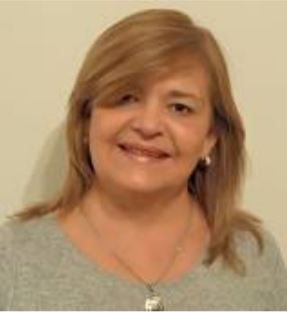
\includegraphics[width=0.2\textwidth]{./fotos/herrera} \end{center} & 
\noindent \small{María Inés Herrera es egresada de la Universidad Nacional de Río Cuarto donde desde 1996 se desempeña como profesora en las Facultades de Cs. Exactas Físico Quimicas y Naturales y de Cs. Económicas, dictando Estadística para diversas carreras y Análisis Matemático. Ha contribuido en distintas iniciativas para promover la Alfabetización estadística (Olimpíadas Estadísticas de Córdoba 2010-2015, preparación del equipo de estudiantes argentinos que participaron en la Competencia Internacional Estadística ISLP Sudáfrica 2009, capacitación de profesores en programas del Ministerio de Ciencia y Tecnología de la Provincia de Córdoba y del Ministerio de Educación y en el marco del Proyecto de Mejora de Formación en Ciencias Exactas y Naturales en la Escuela Secundaria (SPU, 2014-2016). Su formación académica de grado es en Matemática y en posgrado, en Estadística con orientación al Diseño Experimental (UNRC), en Estadística e Investigación Operativa (UPC- España) y en Investigación en la Enseñanza y Aprendizaje de las Ciencias Experimentales, Sociales y Matemáticas (UNIA-España). Ha participado en proyectos de investigación sobre Educación Estadística como así también, en proyectos de Innovación, de Extensión, de Voluntariado Universitario y de Prácticas Socio-comunitarias. Su línea de investigación reciente abarca el estudio de potencialidades y limitaciones de recursos como medios para favorecer el conocimiento didáctico-estadístico.} \\
\end{tabular}
\end{table}


 %--------------------------------------------------------------------------
\newpage
\clearpage
\renewcommand{\titulo}{ESTADÍSTICAS OFICIALES: EMPODERAMIENTO Y VISIBILIDAD DE LAS CUESTIONES SOCIALES}
\renewcommand{\presentador}{DRA. MARCIA QUINTSLR}
\renewcommand{\lugar}{INSTITUTO BRASILEIRO DE GEOGRAFIA E ESTADÍSTICA, BRASIL}
\addcontentsline{toc}{subsubsection}{\titulo. \presentador}
\vspace*{1cm}

\begin{center}
\textbf{\textcolor{ultramarine}{\titulo \\}}
\bigskip
\textit{\presentador \\}
\bigskip
\scriptsize{\lugar}
\bigskip
\end{center}

\noindent Las acciones y reflexiones en la conducción estratégica y política de los Sistemas Estadísticos Nacionales (SENs) implican abordar interlocuciones con diversas instituciones y actores sociales, en las que se expresan tensiones y sinergias que permean todas las etapas del ciclo estadístico. Las interlocuciones, que son de amplio espectro, se configuran en forma de demandas de estadísticas en el proceso de definición del contenido de los programas estadísticos oficiales. Estos programas corresponden a los temas que son investigados por las agencias integrantes del SEN. Indican la visibilidad proporcionada por las estadísticas oficiales a los diferentes temas sociales, económicos, ambientales y a sectores de población o territoriales. Tal visibilidad se desea porque corresponde a información, que resulta en empoderamiento para variados contextos. Las estadísticas sirven para acciones de política pública, para el ejercicio de la ciudadanía, para la toma de decisiones en el campo privado corporativo o personal y para muchas otras finalidades. Se espera de los gestores del SEN una disposición permanente para dialogar conlos interlocutores, teniendo en cuenta los recursos disponibles y las condiciones sociales que limitan la atención de los diversos intereses presentados.

\begin{table}[H]
\centering
\begin{tabular}{m{0.25\textwidth}  m{0.7\textwidth}}
\begin{center} 
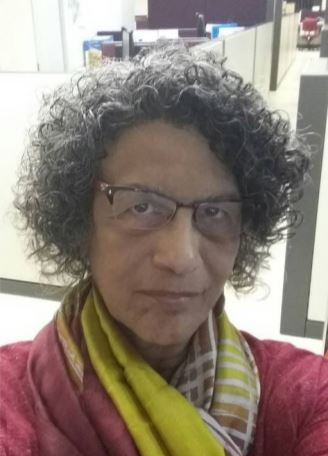
\includegraphics[width=0.2\textwidth]{./fotos/marcia} \end{center} & 
\noindent \small{Marcia Quintslr es brasileña, tiene experiencia en el diseño, planeamiento, producción, análisis y gestión en Estadísticas Oficiales. En el Instituto Brasileño de Geografía y Estadística (IBGE) actuó, desde octubre de 2011 hasta abril de 2014, coordinando la Dirección de Encuestas del Instituto, área responsable por el plan estadístico brasileño y por la Coordinación de las Encuestas de Hogares (2006-2011). Su formación académica es en matemática – ciencia de la computación, con posgrado en estadística. Actualmente está cursando una Maestría en Ciencia de la Información en el Instituto Brasileiro de Ciência e Tecnologia y Universidade Federal do Rio de Janeiro, donde realiza investigación sobre estadísticas, política de información, poder y representación del
conocimiento sobre la sociedad.} \\
\end{tabular}
\end{table}



 %--------------------------------------------------------------------------
\newpage
\clearpage
\renewcommand{\titulo}{ANÁLISIS BAYESIANO DE PARÁMETROS EN ECUACIONES EN DERIVADAS PARCIALES LINEALES}
\renewcommand{\presentador}{DR. MARCO SCAVINO}
\renewcommand{\lugar}{UNIVERSIDAD NACIONAL DE LA REPÚBLICA, URUGUAY}
\addcontentsline{toc}{subsubsection}{\titulo. \presentador}
\vspace*{1cm}

\begin{center}
\textbf{\textcolor{ultramarine}{\titulo \\}}
\bigskip
\textit{\presentador \\}
\bigskip
\scriptsize{\lugar}
\bigskip
\end{center}

\noindent El análisis de las características de aislamiento térmico de materiales y componentes en el sector de la construcción y en las aplicaciones industriales requiere llevar a cabo experimentos cuyos resultados proporcionan información para la estimación de parámetros físicos tales como la conductividad térmica. Desde el punto de vista de la modelación matemática, los parámetros de interés aparecen como coeficientes desconocidos en ecuaciones en derivadas parciales lineales, tales como la ecuación del calor en presencia de ciertas condiciones iniciales y de frontera. En esta charla se presenta un método de inferencia bayesiana para la estimación de parámetros en ecuaciones en derivadas parciales lineales, y su aplicación a un estudio experimental llevado a cabo en una cámara ambiental con el propósito de inferir las propiedades térmicas de una pared. Nuestra técnica de marginalización de las condiciones de frontera reduce el error de sesgo de las estimaciones de los parámetros de la pared en comparación con otros enfoques donde las condiciones de frontera se suponen no aleatorias. Finalmente, el cálculo de la ganancia de información permite orientar al usuario en la determinación eficiente de las variables que caracterizan al experimento.

\begin{table}[H]
\centering
\begin{tabular}{m{0.25\textwidth}  m{0.7\textwidth}}
\begin{center} 
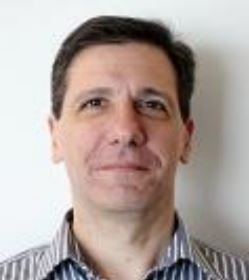
\includegraphics[width=0.2\textwidth]{./fotos/scavino} \end{center} & 
\noindent \small{Licenciado en Ciencias Estadísticas y Demográficas (Università degli Studi di Roma “La Sapienza”, Italia). Doctor en Estadística (Università degli Studi di Padova, Italia). Profesor Agregado efectivo en el Instituto de Estadística de la Facultad de Ciencias Económicas y de Administración de la
Universidad de la República (UdelaR), Montevideo, Uruguay. Se ha desempeñado como coordinador de la Maestría en Ingeniería Matemática (UdelaR) y como Profesor Agregado visitante en King Abdullah University of Science and Technology (KAUST), Arabia Saudita. Ha dictado numerosos cursos de estadística, probabilidad y matemática para carreras de grado y posgrado de Estadística, Ingeniería, Ingeniería Matemática, Bioinformática en UdelaR y en ORT, y para el programa de Matemática Aplicada y Ciencias de la Computación en KAUST. Socio fundador de la Sociedad Uruguaya de Estadística, actualmente vicepresidente. Investigador SNI. Sus líneas de trabajo recientes abarcan tópicos en el diseño de experimentos desde una perspectiva bayesiana, calibración y validación de modelos matemático-estadísticos para la predicción de la vida de fatiga de materiales metálicos, procesos estocásticos y sus aplicaciones.} \\
\end{tabular}
\end{table}

%--------------------------------------------------------------------------





\newpage
\clearpage
\renewcommand{\titulo}{ALFABETIZACIÓN Y CULTURA ESTADÍSTICA DE LOS PROFESORES: ¿UN LOGRO O UNA NECESIDAD?}
\renewcommand{\presentador}{DRA. LILIANA TAUBER}
\renewcommand{\lugar}{UNIVERSIDAD NACIONAL DEL LITORAL, ARGENTINA}
\addcontentsline{toc}{subsubsection}{\titulo. \presentador}
\vspace*{1cm}

\begin{center}
\textbf{\textcolor{ultramarine}{\titulo \\}}
\bigskip
\textit{\presentador \\}
\bigskip
\scriptsize{\lugar}
\bigskip
\end{center}

\noindent La experiencia de trabajar, en el periodo 2014-2017, como autora y responsable de contenido del módulo de Enseñanza de la Probabilidad y la Estadística, en el marco de la Especialización Docente de Nivel Superior en Enseñanza de la Matemática en la Educación Secundaria, ofrecida de manera virtual por el INFD (Instituto Nacional de Formación Docente), buscando promover el desarrollo del sentido estadístico mediante la elaboración de proyectos que pongan en práctica las relaciones entre ideas estocásticas fundamentales, ha permitido la reflexión sobre las prácticas docentes que comúnmente se adoptan a la hora de enseñar Estadística. Asimismo, ha permitido poner al descubierto los desafíos de resignificar los conocimientos presentes en el currículo de Estadística. El análisis de algunas de estas prácticas, sugiere la necesidad de atender a la comprensión gradual sobre la intuición y la formalización en la enseñanza de la Estadística y la Probabilidad. Es por ello que nos interesa exponer y debatir sobre los alcances y las debilidades de la formación docente en lo que respecta a la enseñanza de la disciplina, desde el punto de vista epistemológico y didáctico.

\begin{table}[H]
\centering
\begin{tabular}{m{0.25\textwidth}  m{0.7\textwidth}}
\begin{center} 
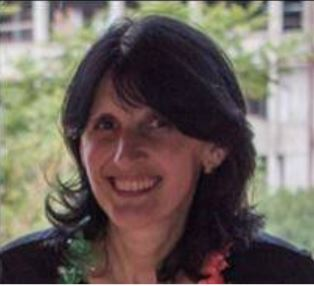
\includegraphics[width=0.2\textwidth]{./fotos/tauber} \end{center} & 
\noindent \small{Liliana Tauber, es Profesora en Matemática, egresada de la Universidad Nacional del Litoral y Doctora en Didáctica de la Matemática por la Universidad de Sevilla. El tema de su Tesis doctoral ha sido: “La Construcción del Significado de la Distribución Normal a partir de actividades de análisis de datos”. Se ha desempeñado como Profesora Titular de Estadística y Métodos Cuali-Cuantitativos en la Carrera de Licenciatura en Psicología de la Universidad Católica de Santa Fe. Desde 1994, se ha desempeñado como profesora de Estadística para diversas carreras, en la Facultad de Humanidades y Ciencias de la Universidad Nacional del Litoral, en la cual actualmente es Profesora Titular. Se especializa en la investigación sobre Educación Estadística, área en la cual ha sido directora de diversos proyectos de investigación desde 2003.} \\
\end{tabular}
\end{table}

 %--------------------------------------------------------------------------

\newpage
\clearpage
\renewcommand{\titulo}{ENSEÑANDO ESTADÍSTICA HOY}
\renewcommand{\presentador}{DRA. TERESITA TERÁN}
\renewcommand{\lugar}{UNIVERSIDAD NACIONAL DE ROSARIO, ARGENTINA}
\addcontentsline{toc}{subsubsection}{\titulo. \presentador}
\vspace*{1cm}

\begin{center}
\textbf{\textcolor{ultramarine}{\titulo \\}}
\bigskip
\textit{\presentador \\}
\bigskip
\scriptsize{\lugar}
\bigskip
\end{center}

\noindent La importancia de la educación estadística, como se observa en todos los niveles de educación en el mundo actual, crece día a día, ya que está ligada al desarrollo de la Estadística como ciencia y a su utilidad en la investigación, la técnica, la vida profesional y el avance de la tecnología plasmada en la potencia de las computadoras y las formas cada vez más rápidas de recibir información. La alfabetización estadística es una necesidad de la sociedad vertiginosa en la que vivimos y es desde la educación estadística que debe ser puesta en marcha en beneficio de la sociedad de la información en la que estamos inmersos. Es por ello que, como docentes de Estadística, se plantea el desafío de cómo enseñar estadística logrando incorporar el pensamiento estadístico a partir de la definición de Moore como aquel que reconoce que la variación está entre nosotros y se presenta en todo lo que hacemos. Se presenta una breve reseña de las Asociaciones que apoyan y fomentan la Educación Estadística, algunas experiencias realizadas en Argentina y en otros países, en diferentes niveles, desde el jardín de infantes hasta la alfabetización de adultos mayores. 

\begin{table}[H]
\centering
\begin{tabular}{m{0.25\textwidth}  m{0.7\textwidth}}
\begin{center} 
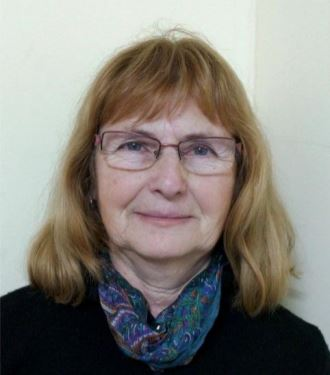
\includegraphics[width=0.2\textwidth]{./fotos/teran} \end{center} & 
\noindent \small{Teresita Terán es Estadística, Profesora en Estadística y Doctora del Programa de Consolidación Académica de la Universidad Nacional de Rosario.
Actualmente es Vicepresidenta del IASE (Asociación Internacional de Educación Estadística). Desde el año 1977 se ha desempeñado como profesora de Estadística, en Institutos Superiores y universitarios. Actualmente es Profesora titular de Bioestadística en la Facultad de Ciencias Veterinarias y de Currículum y Didáctica
y Residencia en el Profesorado en Estadística que se dicta en la Facultad de Humanidades y Artes, dependientes de la UNR. Se ha orientado en forma permanente hacia su especialización en educación matemática y estadística, habiendo realizado en forma continua estudios y participado en seminarios, cursos, talleres, en el área de educación; siendo integrante y luego Directora de grupos de investigación sobre esta temática. Realizó cursos de  perfeccionamiento sobre Pedagogía en Estados Unidos con una Beca Fulbright. Es evaluadora de revistas internacionales, dirige Tesis de Doctorado y ha sido jurado de concursos docentes, tesis de Maestrías y doctorados. Asimismo ha participado en Comisiones evaluadoras de Carrera docente, Acreditación de Carreras de Grado y Posgrado. Escribió varios libros junto con Ana Craveri sobre Estadística Descriptiva, Probabilidad e Inferencia Estadística con aplicaciones en las Ciencias Veterinarias} \\
\end{tabular}
\end{table}
 %--------------------------------------------------------------------------



 